%-----------------------------------------------------------------------------
%
%               Template for sigplanconf LaTeX Class
%
% Name:         sigplanconf-template.tex
%
% Purpose:      A template for sigplanconf.cls, which is a LaTeX 2e class
%               file for SIGPLAN conference proceedings.
%
% Author:       Paul C. Anagnostopoulos
%               Windfall Software
%               978 371-2316
%               paul@windfall.com
%
% Created:      15 February 2005
%
%-----------------------------------------------------------------------------


\documentclass[preprint]{sigplanconf}

% The following \documentclass options may be useful:
%
% 10pt          To set in 10-point type instead of 9-point.
% 11pt          To set in 11-point type instead of 9-point.
% authoryear    To obtain author/year citation style instead of numeric.

\usepackage{amsmath}
\usepackage{listings}
\usepackage{tikz}

\begin{document}

\conferenceinfo{WXYZ '05}{date, City.} 
\copyrightyear{2005} 
\copyrightdata{[to be supplied]} 

\titlebanner{banner above paper title}        % These are ignored unless
\preprintfooter{short description of paper}   % 'preprint' option specified.

\title{Title Text}
\subtitle{Subtitle Text, if any}

\authorinfo{Name1}
           {Affiliation1}
           {Email1}
\authorinfo{Name2\and Name3}
           {Affiliation2/3}
           {Email2/3}

\maketitle

\begin{abstract}
This is the text of the abstract.
\end{abstract}

\category{CR-number}{subcategory}{third-level}

\terms
term1, term2

\keywords
keyword1, keyword2

\section{Introduction}

The text of the paper begins here.

\newpage

foo

\newpage

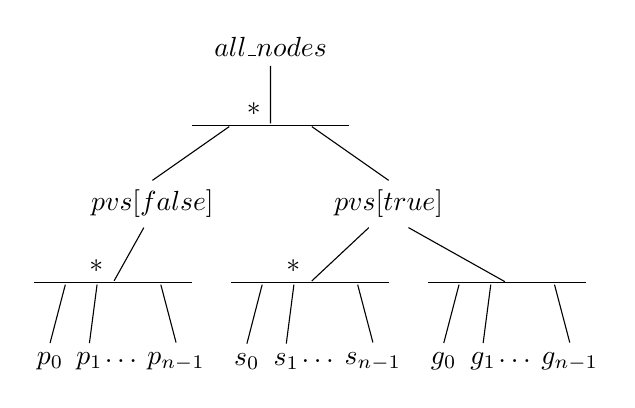
\begin{tikzpicture}
%\draw[step=0.5,gray,very thin] (0,0) grid (8,5);

\node(top) at (3.5,4.5) { $all{\_}nodes$ };

\node(pvsf) at (2,2.5) { $pvs[false]$ };
\node(pvst) at (5,2.5) { $pvs[true]$ };

\node(p0) at (0.7,0.5) { $p_0$ };
\node(p1) at (1.2,0.5) { $p_1$ };
\node(pd) at (1.6,0.5) { $\ldots$ };
\node(pn) at (2.3,0.5) { $p_{n-1}$ };

\node(s0) at (3.2,0.5) { $s_0$ };
\node(s1) at (3.7,0.5) { $s_1$ };
\node(sd) at (4.1,0.5) { $\ldots$ };
\node(sn) at (4.8,0.5) { $s_{n-1}$ };

\node(g0) at (5.7,0.5) { $g_0$ };
\node(g1) at (6.2,0.5) { $g_1$ };
\node(gd) at (6.6,0.5) { $\ldots$ };
\node(gn) at (7.3,0.5) { $g_{n-1}$ };

\draw[xshift=3.5cm,yshift=3.5cm] (-1,0) -- (1,0)
  node[pos=0.25,inner sep=0] {} edge (pvsf.north)
  node[pos=0.5,anchor=south east] {$*$}
  node[pos=0.5,inner sep=0] {} edge (top.south)
  node[pos=0.75,inner sep=0] {} edge (pvst.north)
  ;

\draw[xshift=1.5cm,yshift=1.5cm] (-1,0) -- (1,0)
  node[pos=0.2,inner sep=0] {} edge (p0.north)
  node[pos=0.4,inner sep=0] {} edge (p1.north)
  node[pos=0.5,anchor=south east] {$*$}
  node[pos=0.5,inner sep=0] {} edge (pvsf.250)
  node[pos=0.8,inner sep=0] {} edge (pn.north)
  ;

\draw[xshift=4cm,yshift=1.5cm] (-1,0) -- (1,0)
  node[pos=0.2,inner sep=0] {} edge (s0.north)
  node[pos=0.4,inner sep=0] {} edge (s1.north)
  node[pos=0.5,anchor=south east] {$*$}
  node[pos=0.5,inner sep=0] {} edge (pvst.230)
  node[pos=0.8,inner sep=0] {} edge (sn.north)
  ;

\draw[xshift=6.5cm,yshift=1.5cm] (-1,0) -- (1,0)
  node[pos=0.2,inner sep=0] {} edge (g0.north)
  node[pos=0.4,inner sep=0] {} edge (g1.north)
  node[pos=0.5,anchor=south east] {}
  node[pos=0.5,inner sep=0] {} edge (pvst.310)
  node[pos=0.8,inner sep=0] {} edge (gn.north)
  ;

\end{tikzpicture}

\newcommand{\mygraph}{
%\draw[step=0.5,gray,very thin] (0,0) grid (8,5);

\node[cn,s0] (n1) at (0.77,1.27) {};
\node[cn,p0] (n2) at (1.6165,3.3865) {};
\node[cn,s0] (n3) at (2.463,2.54) {};
\node[cn,p0] (n4) at (0.8755,2.54) {};
\node[cn,p2] (n5) at (2.463,0.529) {};
\node[cn,s2] (n6) at (3.945,1.799) {};
\node[cn,s0] (n7) at (3.6275,2.963) {};
\node[cn,p2] (n8) at (4.7915,0.529) {};
\node[cn,s1] (n9) at (5.638,1.5875) {};
\node[cn,s1] (n10) at (6.6965,1.164) {};
\node[cn,s1] (n11) at (5.215,2.6455) {};
\node[cn,p1] (n12) at (6.379,2.7515) {};
\node[cn,p1] (n13) at (5.3205,3.598) {};
\node[cn,s1,g0] (n14) at (4.1565,4.1275) {};
\node[cn,s0] (n15) at (2.8865,3.81) {};
\node[cn,p0] (n16) at (0.77,4.1275) {};
\node[cn,s2,g0] (n17) at (1.405,0.423) {};
\node[cn,p1] (n18) at (6.379,4.0215) {};
\node[cn,s2,g0] (n19) at (2.7805,1.4815) {};
\node[cn,s0] (n20) at (1.7225,1.799) {};
\node[cn,p2] (n21) at (3.733,0.7405) {};
\node[cn,s2] (n22) at (5.85,0.635) {};

\draw (n16) to (n2);
\draw (n16) to (n4);
\draw (n5) to (n21);
\draw (n21) to (n8);
\draw (n12) to (n13) to (n18) to (n12);


\draw[p2s] (n1) to (n4) to (n20);
\draw[p2s] (n4) to (n3) to (n15) to (n2);
\draw[p2s] (n15) to (n7);

\draw[p2s] (n14) to (n13) to (n11) to (n9) to (n12) to (n10);

\draw[p2s] (n17) to (n19) to (n5);
\draw[p2s] (n19) to (n6) to (n8) to (n22);

\draw[s2s] (n1) to (n17);
\draw[s2s] (n20) to (n19) to (n3);
\draw[s2s] (n15) to (n14) to (n7);
\draw[s2s] (n11) to (n6) to (n9) to (n22) to (n10);

\draw[thick] (0.5,0.5) to (4,2.5);
\draw[thick] (3.75,4.5) to (4,2.5);
\draw[thick] (6.5,0.5) to (4,2.5);

\draw[dashed] (0.5,2) .. controls (1,2) and (1.5,2.5) .. (1.9,3.1) .. controls (2,4) .. (1.75,4.5);
\draw[dashed] (5.25,4.5) .. controls (4.75,3.5) .. (5.25,3.25) .. controls (6,3) .. (6.25,2.5) .. controls (6.25,2.25) .. (7,2);
\draw[dashed] (2,0.25) .. controls (2.25,1) .. (3.5,1.1) .. controls (5,1.25) .. (5.5,0.25);
}

\begin{tikzpicture}
  [cn/.style={circle,draw,minimum size=2mm},
   p0/.style={fill},
   p1/.style={fill},
   p2/.style={fill},
   s0/.style={fill=lightgray},
   s1/.style={fill=lightgray},
   s2/.style={fill=lightgray},
   g0/.style={},
   p2p/.style={very thin},
   p2s/.style={very thin},
   s2s/.style={very thin}]
\mygraph
\end{tikzpicture}

\begin{tikzpicture}
  [cn/.style={circle,draw,minimum size=2mm},
   p0/.style={fill},
   p1/.style={},
   p2/.style={},
   s0/.style={},
   s1/.style={},
   s2/.style={},
   g0/.style={},
   p2p/.style={very thin},
   p2s/.style={very thin},
   s2s/.style={very thin}]
\mygraph
\end{tikzpicture}

\begin{tikzpicture}
  [cn/.style={circle,draw,minimum size=2mm},
   p0/.style={},
   p1/.style={},
   p2/.style={},
   s0/.style={fill},
   s1/.style={},
   s2/.style={},
   g0/.style={},
   p2p/.style={very thin},
   p2s/.style={very thin},
   s2s/.style={very thin}]
\mygraph
\end{tikzpicture}

\begin{tikzpicture}
  [cn/.style={circle,draw,minimum size=2mm},
   p0/.style={},
   p1/.style={},
   p2/.style={},
   s0/.style={fill},
   s1/.style={},
   s2/.style={},
   g0/.style={fill},
   p2p/.style={very thin},
   p2s/.style={very thin},
   s2s/.style={very thin}]
\mygraph
\end{tikzpicture}

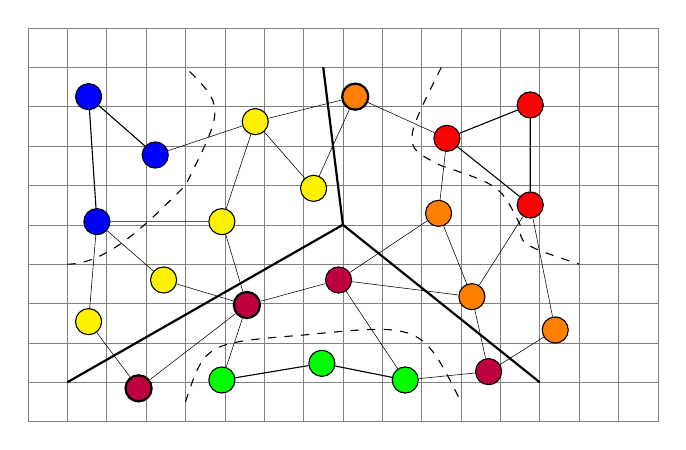
\begin{tikzpicture}
  [cn/.style={circle,draw,minimum size=2mm},
   p0/.style={fill=blue},
   p1/.style={fill=red},
   p2/.style={fill=green},
   s0/.style={fill=yellow},
   s1/.style={fill=orange},
   s2/.style={fill=purple},
   g0/.style={thick},
   p2p/.style={very thin},
   p2s/.style={very thin},
   s2s/.style={very thin}]
\draw[step=0.5,gray,very thin] (0,0) grid (8,5);

\node[cn,s0] (n1) at (0.77,1.27) {};
\node[cn,p0] (n2) at (1.6165,3.3865) {};
\node[cn,s0] (n3) at (2.463,2.54) {};
\node[cn,p0] (n4) at (0.8755,2.54) {};
\node[cn,p2] (n5) at (2.463,0.529) {};
\node[cn,s2] (n6) at (3.945,1.799) {};
\node[cn,s0] (n7) at (3.6275,2.963) {};
\node[cn,p2] (n8) at (4.7915,0.529) {};
\node[cn,s1] (n9) at (5.638,1.5875) {};
\node[cn,s1] (n10) at (6.6965,1.164) {};
\node[cn,s1] (n11) at (5.215,2.6455) {};
\node[cn,p1] (n12) at (6.379,2.7515) {};
\node[cn,p1] (n13) at (5.3205,3.598) {};
\node[cn,s1,g0] (n14) at (4.1565,4.1275) {};
\node[cn,s0] (n15) at (2.8865,3.81) {};
\node[cn,p0] (n16) at (0.77,4.1275) {};
\node[cn,s2,g0] (n17) at (1.405,0.423) {};
\node[cn,p1] (n18) at (6.379,4.0215) {};
\node[cn,s2,g0] (n19) at (2.7805,1.4815) {};
\node[cn,s0] (n20) at (1.7225,1.799) {};
\node[cn,p2] (n21) at (3.733,0.7405) {};
\node[cn,s2] (n22) at (5.85,0.635) {};

\draw (n16) to (n2);
\draw (n16) to (n4);
\draw (n5) to (n21);
\draw (n21) to (n8);
\draw (n12) to (n13) to (n18) to (n12);


\draw[p2s] (n1) to (n4) to (n20);
\draw[p2s] (n4) to (n3) to (n15) to (n2);
\draw[p2s] (n15) to (n7);

\draw[p2s] (n14) to (n13) to (n11) to (n9) to (n12) to (n10);

\draw[p2s] (n17) to (n19) to (n5);
\draw[p2s] (n19) to (n6) to (n8) to (n22);

\draw[s2s] (n1) to (n17);
\draw[s2s] (n20) to (n19) to (n3);
\draw[s2s] (n15) to (n14) to (n7);
\draw[s2s] (n11) to (n6) to (n9) to (n22) to (n10);

\draw[thick] (0.5,0.5) to (4,2.5);
\draw[thick] (3.75,4.5) to (4,2.5);
\draw[thick] (6.5,0.5) to (4,2.5);

\draw[dashed] (0.5,2) .. controls (1,2) and (1.5,2.5) .. (2,3) .. controls (2.5,4) .. (2,4.5);
\draw[dashed] (5.25,4.5) .. controls (4.75,3.5) .. (5.25,3.25) .. controls (6,3) .. (6.25,2.5) .. controls (6.25,2.25) .. (7,2);
\draw[dashed] (2,0.25) .. controls (2.25,1) .. (3.5,1.1) .. controls (5,1.25) .. (5.5,0.25);
\end{tikzpicture}

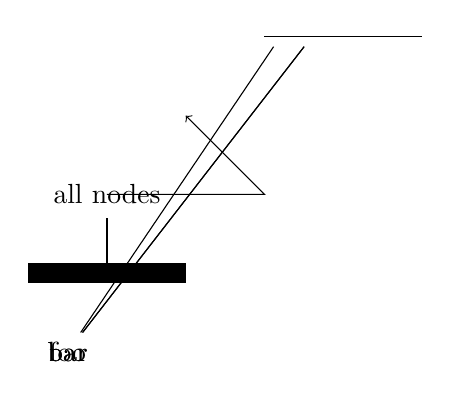
\begin{tikzpicture}

\draw[->] (0,0) -- (2cm,0) -- (1cm,1cm);
\node[inner sep=5pt] (all nodes) at (0,0) {all nodes};
\node (p1) at (0,-1) [shape=rectangle,fill=black,minimum width=2cm,draw] {}
  edge (all nodes);
\draw[xshift=3cm,yshift=2cm] (-1,0) -- (1,0)
  node(n1)[pos=0.1] {}
  node(n2)[pos=0.3] {}
  node(n3)[pos=0.5] {}
  node(n4)[pos=0.7] {}
  node(n5)[pos=0.9] {};
\node (r1) at (-0.5,-2) {foo}
  edge (n1);
\node (r2) at (-0.5,-2) {bar}
  edge (n2);
\node (r2) at (-0.5,-2) {bar}
  edge (n2);
\end{tikzpicture}


\newpage

\lstset{
  captionpos=b,
  language=C++,
  basicstyle=\scriptsize,
  numbers=left,
  numberstyle=\tiny,
  columns=fullflexible,
  stepnumber=1,
  escapechar=\#,
  keepspaces=true,
  literate={<}{{$\langle$}}1 {>}{{$\rangle$}}1,
  morekeywords={region_relation,region,coloring,partition,spawn},
  deletekeywords=float,
}
\begin{lstlisting}[float={t},label={lst:code_ex},caption={Circuit Simulation Code Example}]
struct Node<rn>    { Node<rn>@rn next;    float charge, capacitance; }
struct Wire<rn,rn2,rw> { Wire<rn,rn2,rw>@rw next;
                                          Node<rn2>@rn in_node, out_node; float current, ... ; }
region_relation Circuit {
  region< Node<r_all_nodes> >                        r_all_nodes;
  region< Wire<r_all_nodes,r_all_nodes,r_all_wires> >       r_all_wires;
  Node<r_all_nodes>@r_all_nodes                   first_node;
  Wire<r_all_nodes,r_all_wires>@r_all_wires   first_wire;
}
region_relation CircuitPiece<rn, rw> {
  region< Node<rn_pvt+rn_shr> >                                 rn_pvt (#$\prec$# rn), rn_shr (#$\prec$# rn);
  region< Node<rn> >                                                   rn_ghost (#$\prec$# rn);
  region< Wire<rn_pvt+rn_shr+rn_ghost,rn,rw_pvt> >  rw_pvt (#$\prec$# rw);
  Node<rn_pvt+rn_shr>@(rn_pvt+rn_shr)                     first_node;
  Wire<rn_pvt+rn_shr+rn_ghost,rn,rw_pvt>@rw_pvt    first_wire;
};
void simulate_circuit(Circuit c) : RWE(c.r_all_nodes,c.r_all_wires)
{
  partition<c.r_all_wires> p_wires(wire_owner_map); // colored by piece they're in
  partition<c.r_all_nodes> p_nodes_pvs(node_sharing_map);
                                                                    // true = some neighbors in other pieces
  partition<p_nodes_pvs[false]> p_pvt_nodes(node_owner_map);
                                                                    // colored by piece they're in
  partition<p_nodes_pvs[true]> p_shr_nodes(node_owner_map);
                                                                    // colored by piece they're in
  partition<p_nodes_pvs[true]> p_ghost_nodes(node_nghbr_map);
                                                                    // colored by pieces they neighbor

  CircuitPiece<c.r_all_nodes,c.r_all_wires> pieces[MAX_PIECES];
  for(i = 0; i #$<$# MAX_PIECES; i++) 
    pieces[i] #$\gets$# { rn_pvt = p_pvt_nodes[i], rn_shr = p_shr_nodes[i],
                            rn_ghost = p_ghost_nodes[i], rw_pvt = p_wires[i] };

  while(!done) {
    for(i = 0; i #$<$# MAX_PIECES; i++) spawn calc_new_currents(pieces[i]);
    for(i = 0; i #$<$# MAX_PIECES; i++) spawn distribute_charge(pieces[i]);
    for(i = 0; i #$<$# MAX_PIECES; i++) spawn update_voltages(pieces[i]);
  }
}

// read info from nodes connected to each wire, update state of wire
void calc_new_currents(CircuitPiece<rn,rw> piece): RWE(piece.rw_pvt),
                                                                         ROE(piece.rn_pvt,piece.rn_ghost)

// current moving through wires redistributes charge between nodes
void distribute_charge(CircuitPiece<rn,rw> piece): ROE(piece.rw_pvt),
                                                                         RdA(piece.rn_pvt,piece.rn_ghost)

// total charge added to a node causes changes in voltage
void update_voltages(CircuitPiece<rn,rw> piece): RWE(piece.rn_pvt,piece.rn_shr)
\end{lstlisting}


\newpage


\newpage

blah

\newpage

blah

\newpage

\section{Low-Level Runtime}
\label{sec:lowlevel}

The low-level runtime is a machine-independent layer that provides portability
to the high-level runtime and consequently the Legion programming model.
The low-level runtime hides the ideosynchracies of the underlying machine while
at the same time not straying 
too far from the native capabilities of the underlying hardware.  
The machine abstraction that the Legion low-level runtime presents is a base set
of objects.  These objects,
include processors, memories, regions, events, and deffered locks.

%The target machines for Legion include both clusters and GPU-equipped nodes,
%and neither of which are able to efficiently provide a uniformly addressable
%and accessible memory space across the system.  The low-level runtime does
%not hide this fact from the high-level runtime, but rather relies on the
%high-level runtime to manage data movement.  Consequently all objects in
%the low-level runtime are named by handles 
%which can be copied by value and moved around the machine.

%The low-level runtime provides a deferred execution model rather
%than the more common immediate model where operations occur as soon
%as requested.  Requests made of the low-level 
%runtime usually return to the caller immediately, with the requested action
%performing asynchronously to the caller's thread of execution.  This is done
%for two different, but equally important, reasons.  First, it matches the
%standard GPU execution model.  GPUs tend to have very deep pipelines, and
%maximum performance cannot be achieved if each command has to be run to
%completion before the next command can be started.  Second, in clusters, the
%latency of inter-node communication can be significant, and a caller that
%waited for every request of a remote node to return before continuing on would
%also be similarly underutilizing the computational resources of the system.

%Although it does not show up explicitly in the interface, the low-level runtime
%was also architected to permit a distributed and hierarchical implementation.
%Critical resources can be replicated or migrated between nodes to reduce
%both average latencies and the amount of traffic that use the scarce inter-node
%communication bandwidth.



\subsection{Low-Level Abstractions}
\label{subsec:lowobjects}
\subsubsection{Events}
\label{subsec:events}
The low-level runtime supports a deffered execution model to hide
the latencies associated with communicating in a distributed memory
system.  The basic building block of the low-level runtime's deferred execution model
is the {\em event}.  An event is a placeholder for the completion of a deferred
operation.  When an asynchronous call is made to any of the low-level runtime objects, an event is 
immediately returned to the caller.  The caller may query whether the event has {\em triggered}
which happens when the operation corresponding to the event completes.  The common use case for events is
to provide them as prerequisites to subsequent requests made of the runtime. 
These dependences cause the later requests to be automatically deferred until the previous
events have triggered.  By using events as dependences, the caller can
set up complicated, but coordinated chains of operations to be executed without
having to wait for the low-level runtime to execute them.
%These requests will
%also return events, and the caller can set up a complicated, but coordinated,
%set of operations to be performed by the low-level runtime with no babysitting
%required of the original caller.

With nearly every single runtime operation creating a new event and referring
to potentially any number of past events, both the time and space overhead of
implementing events is a serious concern.  The time overhead is addressed by a
mechanism that allows a node to create a new event without needing to
communicate with any other node.  The event's handle identifies which node
created it, allowing another node to lazily access it only when and if it 
is asked to perform an operation on it.  Checking to see if an event has
occurred is done via a subscription mechanism.  Any number of threads or
deferred operations on one node can query or wait on an event with a single
message sent to the originating node.  The requesting node tracks the multiple
local requestors and upon receiving the trigger message from the originating
node, distributes that message to all the local parties that are interested.

The potential space concern with events is addressed by a {\em generation scheme}
that allows events to be reclaimed and reused without tracking references.  The
naive implementation of an event cannot reclaim the storage used by an event
until the event has triggered and all waiters on the event have been
notified.  Some of these waiters may take quite a while to query the event.
Additionaly, we must somehow track how many queries to expect to know
when they've all been performed.  However, if the event handle is paired with a
{\em generation count} that tracks how many times the event has been triggered,
the event can be reused as soon as the previous generation has been triggered.
Holders of an older (handle,generation) pair are able to query the newer
incarnation of the event and determine from the generation mismatch that their
event must have already triggered.  With this technique, there is no need to
count references to the event at all. 
% An event can only be reused until the
%generation counter reaches its maximum value, the current implementation
%supports $2^{32}-1$ generations, and should that not be sufficient, extending
%it to $2^{64}-1$ is trivial.

\subsubsection{Deferred Locks}
\label{subsec:defferedlocks}
Events are used to provide a deterministic ordering between operations, but in
some cases are overly restrictive.  To implement the more relaxed coherence
properties supported in Legion we need a less restrictive ordering semantics that
can result in better performance.  The traditional tool for this job is
the mutex (a.k.a. lock), and it is from the common reader/writer lock that
the low-level runtime's {\em deferred lock} is derived.  The key visible 
difference between a mutex and a deferred lock is that the request does not
block the caller's execution.  Many libraries offer nonblocking locks, but
they achieve this by returning without the lock if it is unavailable.  If
a deferred lock is currently unavailable, the request is guaranteed to be
granted at some time in the future (with no further action required of the 
caller).  That time in the future is described with an event.  Like all other
events, it can be given to other threads, or even stored
in a data structure in memory to be extracted by an arbitrary thread at a 
later time.  This dissociation of a held lock from the thread that
requested it is another important difference between the deferred lock and
existing mutexes.

The deferred nature of a deferred lock also allows a distributed implementation
of locks.  Similar to events, a deferred lock can be created on any node
without communication with the other nodes in the cluster.  That node becomes
the initial home for the lock, but the deferred lock (unlike events) can 
migrate to other nodes or even be shared between nodes, allowing repeated
lock requests from a single node to be kept local to that node after a single
message is sent to the current owner.  (Should the ownership of the lock change
while the message is in flight, the previous owner forwards the request to
the new owner.  The highly unlikely, but possible, case in which multiple 
forwardings are required is bounded at the number of nodes in the cluster.)
The ability to migrate locks between nodes allows the performance of a
heavily-contended cluster-level lock to approach that of a single-node lock.

The final interesting feature of the deferred lock is that it can be associated
with an object in memory and that object will automatically be kept coherent
across the cluster.  This is similar to MESI coherence in a distributed cache,
but is done per-object rather than on cache lines.  This is currently only 
used for object within the runtime itself, but we are exploring ways to expose
it at the Legion application level.

\subsubsection{Processors}
\label{subsec:processors}
Hardware units capable of performing computation are captured as generic
processors in the low-level runtime.  Like other runtime objects, a processor
has a globally unique name and can be referred to anywhere in the system.
Processors come in different \emph{kinds} (e.g. X86 CPU core, CUDA-capable GPU),
but they all support the same
interface and execution model.  A request to spawn a task on a given processor
may come from anywhere in the system.  The request names which task should
be spawned and provides input arguments and zero or more events.  Once those
events have occurred, the task is placed into a queue of ready tasks, which
the processor works through in the order in which they were enqueued.  A
processor will generally run a task to completion before taking another, but
will try to run another task (resources permitting) if the current task needs
to wait for an event to occur.  Once a task is placed on a processor's queue,
it may not be moved or deleted.  Load-balancing of tasks is expected to be done
by the high-level runtime.  The primary purpose of the queue for the low-level
Processor is to be able to hide the latency of starting new tasks.

\subsubsection{Memories}
\label{subsec:memories}
Application-visible storage in the low-level runtime is described in terms of
memory objects.  A memory object has a size and describes its affinity to 
processors (and other memories) in terms of relative bandwidth and latency.
The low-level runtime allows for the allocation and freeing of region instances
and allocators.  It also supports bulk transfers from one memory to another.
These bulk transfers can often be implemented using dedicated DMA (or RDMA)
hardware, freeing up the processors to perform more interesting
computation. 

\subsubsection{Regions}
\label{subsec:regionmeta}
Application-level regions are broken into four inter-related pieces in the
low-level runtime:
\begin{description}

\item[MetaData] The metadata for a logical region captures attributes of a
logical region that are common across all instances.  These attributes include
the size of the logical region, the element type, and the allocation mask,
which tracks which portions of the logical region are actually in use.  
%Region
%MetaDatas are created independently of any memory objects and are accessible
%(via a globally unique name) to all nodes in the machine.

\item[Allocator] The dynamic memory allocation capability of a region instance
is provided via an allocator object.  An allocator is associated with a
region metadata and must be created in a particular memory.  Once created, it
may be used to allocate and free elements of the region by any task on any
processor that has non-zero affinity with the memory.

\item[Instance] Each physical instance of a region stores some version of all
the elements in a region.  As with allocators, a physical instance is
associated with a particular region metadata and spends its entire lifetime in
the memory objecy in which it was created.  
%When multiple physical instances
%exist for the same region, the low-level runtime does nothing to keep them
%copies and set up the right inter-operation dependencies to provide the level
%of coherence requested by the application.  Although a physical instance 
%stores the contents of a region, it does not directly offer access to those
%contents.

\item[Accessor] Access to the contents of a physical region instance are 
handled by accessor objects.  These are lightweight objects that allow a given
task to access a given physical region instance, regardless of the
implementation of that instance or the underlying memory.  In the most common
case, read and write access is done through a single array dereference, but the
accessor interface allows seamless use of other types of memory as well (e.g.
memory that's accessed via RMDA put and get calls).

\end{description}


\subsection{Low-Level Implementations}
\label{subsec:lowimpl}
The primary goal of the low-level runtime is to provide an
abstraction that enables efficient execution of Legion programs
on a wide array of machines.  To support this claim we describe
two implementation of the low-level runtime: one based on POSIX
threads for a shared memory SMP and one based on GASNet and CUDA
for distributed memory clusters with multiple GPUs.
%The magic of an
%apparently-unified address space is left to the high-level runtime, and the
%interface to the low-level runtime is done in terms of handles rather than 
%pointers for runtime objects and relative offsets rather than absolute 
%pointers for resource allocations.

%\subsection{Initialization}

%On startup, the low-level runtime allocates all the resources it needs from
%the operating system and set up the communication channels between nodes.
%Each processor in the system then automatically runs the high-level runtime's
%initialization task, which will usually spawn more tasks.  These tasks are
%started, and whenever any processor's task queue is empty , the high-level
%runtime's scheduler task is automatically called to explore the possibility
%of moving tasks around for load balancing.

\subsubsection{SMP Implementation}
\label{subsec:smpimpl}
The SMP implementation of the low-level runs on any SMP machine that supports 
POSIX threads.  A single memory object is created for the shared memory, and 
a processor object is created for
each CPU core in the system.  Events are 
mutex-protected data structures that maintain a list of callbacks to call when
the corresponding event is triggered.  Locks are similar, except that the list
is of pending lock requests to attempt when the previous lock is released.

\subsubsection{GPU Cluster Implementation}
\label{subsec:clusterimpl}
The cluster implementation of the low-level runtime is implemented on a mix
of POSIX threads for intra-node threading and communication, GASnet for 
inter-node communication, and CUDA for access to resources of the GPUs in 
each node.  Locks and events have roughly the same implementation as the SMP
runtime for handling multiple local requestors, but use GASnet active messages
to coordinate lock ownership and event subscription and triggering between
nodes.  In addition to the processor objects for each CPU core, a single
processor object is created for each GPU in the system.  It would be preferable
to expose the GPU's computational resources at a finer granularity, but
current GPU hardware doesn't directly allow this flexibility and recent attempts
at implementing such control in a software layer on top of CUDA have suffered
from significant overhead.  The memory hierarchy is expanded to include a 
{\em global} memory that is striped across all nodes and accessible via GASnet
RDMA calls, one process local memory per cluster node, and two memories per GPU: one for the GPU's framebuffer that is
accessible only to that GPU and by bulk DMA operations, and one for the pinned
{\em zero copy} system memory that is accessible to the GPU and all the CPU cores
in a single system.


\newpage


\appendix
\section{Appendix Title}

This is the text of the appendix, if you need one.

\acks

Acknowledgments, if needed.

% We recommend abbrvnat bibliography style.

\bibliographystyle{abbrvnat}

% The bibliography should be embedded for final submission.

\begin{thebibliography}{}
\softraggedright

\bibitem[Smith et~al.(2009)Smith, Jones]{smith02}
P. Q. Smith, and X. Y. Jones. ...reference text...

\end{thebibliography}

\end{document}
